\section{Results}

\subsection{Five-model diagnostic summary}
\label{sec:results_five_model_summary}

Across 17 stations and seven forecast horizons, direct HGB and Ridge achieve positive RMSE skill in all station-horizon cells but show near-universal variance collapse. HGB collapses in 118/119 cells (99.2\%) and Ridge in 118/119 cells (99.2\%), with only two $h=1$ point-estimate exceptions: Huesca for HGB ($\alpha = 0.544$) and Barcelona Vall d'Hebron for Ridge ($\alpha = 0.502$). SARIMA exhibits a similar but slightly less extreme pattern, collapsing in 110/119 cells (92.4\%). Seasonal naive preserves variance (0/119 collapsed cells) but has slightly negative median skill, whereas STL+Ridge avoids variance collapse but inflates variability and performs substantially worse in RMSE skill. Thus, the observed trade-off is not a simple model ranking problem: models can be significantly skillful in RMSE while dynamically over-smoothed, or dynamically variable while inaccurate.

\begin{landscape}
\begin{table}[p]
\centering
\small
\setlength{\tabcolsep}{5pt}
\caption{Model-family diagnostic summary across 17 stations and seven horizons. Collapse is defined as $\alpha < 0.5$. Near-ideal cells require positive RMSE skill and $\alpha \geq 0.8$. DM counts report BH-adjusted Diebold-Mariano tests against persistence. Exceedance metrics summarize event-detection behaviour across the evaluated thresholds.}
\label{tab:five_model_diagnostic_summary}
\begin{tabular}{llrrrrrrrrr}
\toprule
Model & Family & Med. Skill & Med. $\alpha$ & Collapse \% & Retained \% & Near-Ideal \% & Sig. Imp & Sig. Deg & Med. CSI & Med. FAR \\
\midrule
hgb\_direct & Direct ML & 0.205 & 0.151 & 99.2\% & 0.0\% & 0.0\% & 111 & 0 & 0.121 & 0.647 \\
ridge\_direct & Direct ML & 0.219 & 0.087 & 99.2\% & 0.0\% & 0.0\% & 117 & 0 & 0.104 & 0.595 \\
sarima & Statistical baseline & 0.208 & 0.095 & 92.4\% & 0.0\% & 0.0\% & 44 & 0 & 0.118 & 0.500 \\
seasonal\_naive & Variance-preserving naive & -0.026 & 1.000 & 0.0\% & 98.3\% & 16.8\% & 5 & 34 & 0.111 & 0.822 \\
stl\_ridge\_direct & Decomposition + Ridge & -1.107 & 1.399 & 0.0\% & 100.0\% & 0.0\% & 0 & 119 & 0.104 & 0.896 \\
\bottomrule
\end{tabular}
\end{table}
\end{landscape}


Under the ``near-ideal'' criterion (Skill $>0$ and $\alpha \geq 0.8$), no non-naive evaluated model attains any near-ideal cell: HGB direct, Ridge direct, SARIMA, and STL+Ridge each have 0/119 near-ideal cells. Seasonal naive contributes 20/119 near-ideal cells, but it is a naive reference and should not be interpreted as a superior predictive model.

\subsection{Horizon profiles of skill and variance retention}

To make the multi-horizon behaviour readable in the main text, we summarise horizon profiles using station-wise medians and interquartile ranges (IQR). Figure~\ref{fig:skill_profiles} reports median persistence-relative RMSE skill by horizon, and Figure~\ref{fig:alpha_profiles} reports the corresponding variance-retention ratio $\alpha$. The detailed three-model horizon table used in early diagnostic development is provided in the Supplementary Material.

\begin{figure}[t]
  \centering
  
\includegraphics[width=\linewidth]{figures/figure3_skill_profiles.pdf}
  \caption{Median persistence-relative RMSE skill by forecast horizon across 17 PM$_{10}$ stations. Shaded bands denote interquartile ranges across stations. HGB, Ridge, and SARIMA retain positive median skill, whereas seasonal naive remains close to persistence and STL+Ridge is substantially worse than persistence.}
  \label{fig:skill_profiles}
\end{figure}

\begin{figure}[t]
  \centering
  
\includegraphics[width=\linewidth]{figures/figure4_alpha_profiles.pdf}
  \caption{Median variance-retention ratio by forecast horizon across 17 PM$_{10}$ stations. The grey region indicates collapsed variance ($\alpha < 0.5$), and the green band indicates near-retained variance. HGB, Ridge, and SARIMA rapidly enter the collapsed region, while seasonal naive remains close to $\alpha = 1$ and STL+Ridge preserves or inflates variance.}
  \label{fig:alpha_profiles}
\end{figure}

\subsection{Skill--$\alpha$ diagnostic space}

Figure~\ref{fig:skill_alpha_space} provides a single-reading diagnostic summary of the skill--fidelity trade-off (cf. joint-performance summaries in \cite{taylor2001}).

\begin{figure}[t]
  \centering
  
\includegraphics[width=\linewidth]{figures/figure5_scatter_skill_alpha.pdf}
  \caption{Skill-retention diagnostic by model. Points show model-level medians across station-horizon cells, and error bars show interquartile ranges. HGB, Ridge, and SARIMA occupy the skillful-but-collapsed region, seasonal naive lies near retained variance but near-zero skill, and STL+Ridge preserves or inflates variance while losing RMSE skill.}
  \label{fig:skill_alpha_space}
\end{figure}

\subsection{SARIMA and STL+Ridge as diagnostic controls}

SARIMA and STL+Ridge were included to test whether the skill--variance trade-off is specific to direct lag-only ML. SARIMA behaves similarly to HGB and Ridge: it obtains positive median RMSE skill (0.208) but collapses in 110/119 cells (92.4\%). STL+Ridge provides the opposite control case. It avoids variance collapse in all cells and has median $\alpha = 1.399$, but its median RMSE skill is strongly negative ($-1.107$) and all 119 station-horizon cells are significantly worse than persistence under the BH-adjusted DM test. This result shows that preserving amplitude is necessary but not sufficient: the retained variability must also be phase-aligned and forecast-relevant.

\subsection{Sensitivity to the $\alpha$ threshold}

The conclusion is robust to threshold perturbations. At $\alpha < 0.4$, HGB and Ridge still collapse in 92.4\% and 89.9\% of cells, respectively; at $\alpha < 0.5$ both collapse in 99.2\%; and at $\alpha < 0.6$ both collapse in 100.0\%. SARIMA also remains highly collapsed across this range (89.9\%, 92.4\%, and 96.6\%, respectively). Seasonal naive and STL+Ridge remain non-collapsed at these thresholds. The threshold $\alpha = 0.5$ is therefore not driving the qualitative conclusion, although it should be interpreted as a diagnostic convention rather than a universal physical boundary.

\begin{figure}[t]
  \centering
  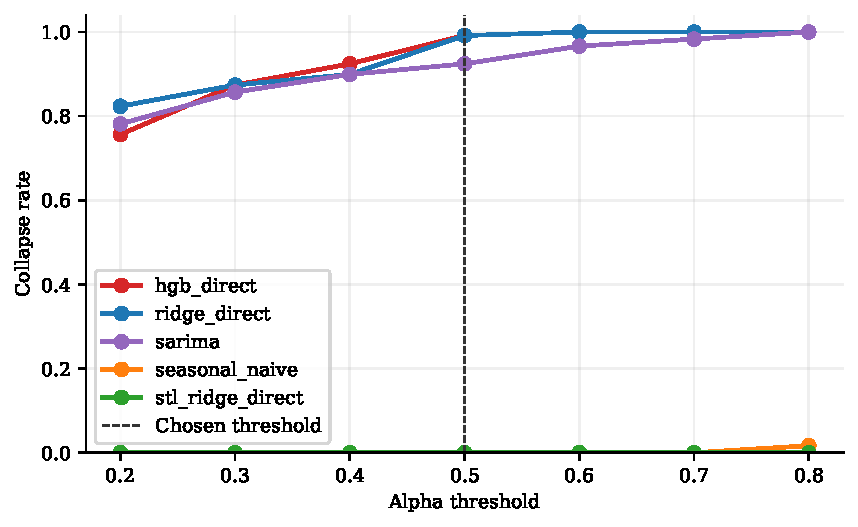
\includegraphics[width=\linewidth]{figures/figure_threshold_sensitivity.pdf}
  \caption{Sensitivity of the variance-collapse diagnostic to the $\alpha$ threshold. Collapse remains near-universal for HGB and Ridge across reasonable thresholds around $\alpha = 0.5$, and SARIMA follows the same qualitative pattern. Seasonal naive and STL+Ridge remain non-collapsed over the same range, showing that the diagnostic separates smoothed forecasts from variance-preserving or variance-inflating alternatives.}
  \label{fig:threshold_sensitivity}
\end{figure}

\subsection{Diebold--Mariano significance against persistence}

The RMSE gains of the smoothed models are not merely sampling noise. Relative to persistence, the BH-adjusted Diebold--Mariano tests (paired squared losses with the Harvey--Leybourne--Newbold correction \cite{harvey1997}) identify significant improvements in 111/119 HGB cells and 117/119 Ridge cells. SARIMA is significantly better in 44/119 cells. In contrast, STL+Ridge is significantly worse in all 119 cells. These tests make the central paradox explicit: statistically significant RMSE improvements can coexist with severe loss of predictive variance and poor event sensitivity.

\subsection{Operational consequence: exceedance behaviour}

The operational consequence of variance collapse is visible in event detection. For P75 events, mean recall is 26.9\% for HGB, 21.0\% for Ridge, and 15.6\% for SARIMA, compared with 40.0\% for persistence and 32.6\% for seasonal naive. At P90, recall falls to 7.4\%, 5.6\%, and 6.9\%, respectively. STL+Ridge achieves much higher recall (98.4\% at P75 and 87.7\% at P90), but with low precision (mean 24.2\% at P75) and high false-alarm rates. Thus, neither RMSE skill nor variance retention alone is sufficient for operational forecasting: the evaluation must jointly consider amplitude, event detection, and false alarms.

\begin{figure}[t]
  \centering
  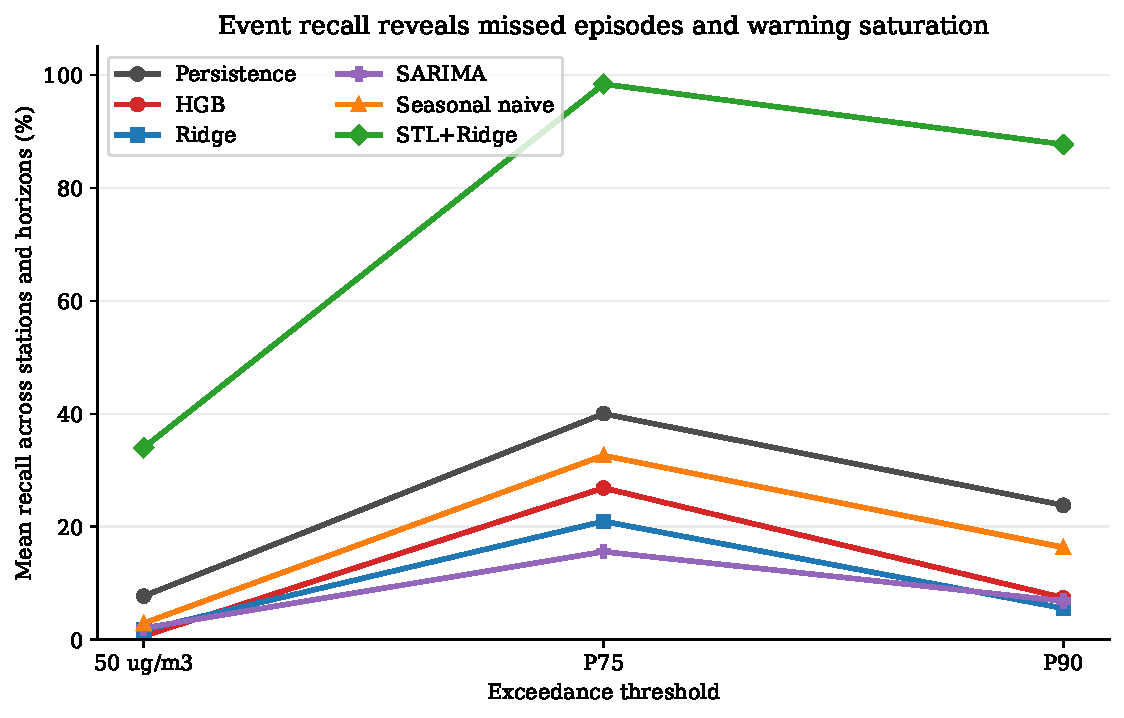
\includegraphics[width=\linewidth]{figures/figure_exceedance_recall.pdf}
  \caption{Mean exceedance recall across stations and horizons. Despite positive RMSE skill, HGB, Ridge, and SARIMA miss many P75 and P90 events. STL+Ridge attains high recall, but this must be interpreted together with its low precision and high false-alarm rate.}
  \label{fig:exceedance_recall}
\end{figure}

\subsection{Murphy decomposition}

The Murphy decomposition links the empirical findings to forecast verification theory \cite{murphy1988}. The smoothed models reduce error while compressing predictive variability, whereas STL+Ridge preserves or inflates variability but introduces large error components. This decomposition supports the interpretation that the main failure mode is not simple unconditional bias but a mismatch between forecast amplitude, phase, and conditional structure.

\begin{figure}[t]
  \centering
  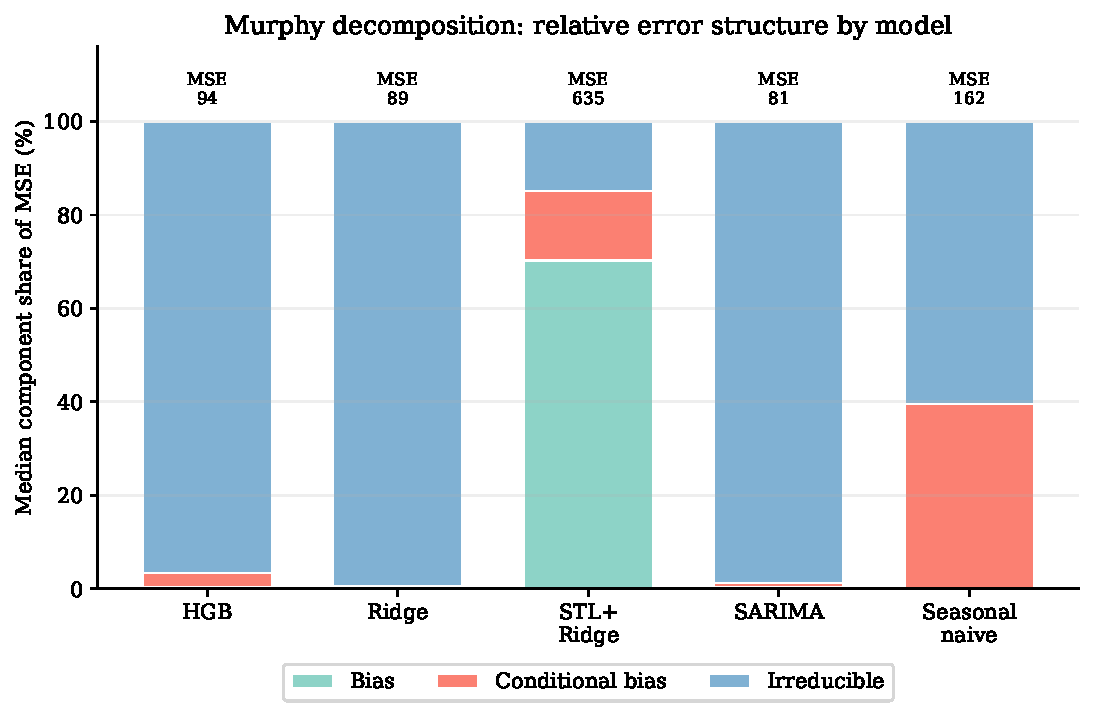
\includegraphics[width=\linewidth]{figures/figure_murphy_decomposition.pdf}
  \caption{Murphy decomposition of mean squared error by model. Bars show median percentage contribution of bias, conditional bias, and irreducible components; labels above bars report median MSE. The decomposition shows that variance preservation alone does not guarantee useful deterministic forecasts.}
  \label{fig:murphy_decomposition}
\end{figure}

\subsection{Cross-station consistency and station heterogeneity}
\label{E3}

The station set is heterogeneous, including urban traffic, urban/background, suburban industrial, rural remote/background, and EMEP sites. Figure~\ref{fig:station_map_ml_only} shows the geographic distribution and confirms that variance collapse in direct ML is nearly ubiquitous across station types.

\begin{figure}[t]
  \centering
  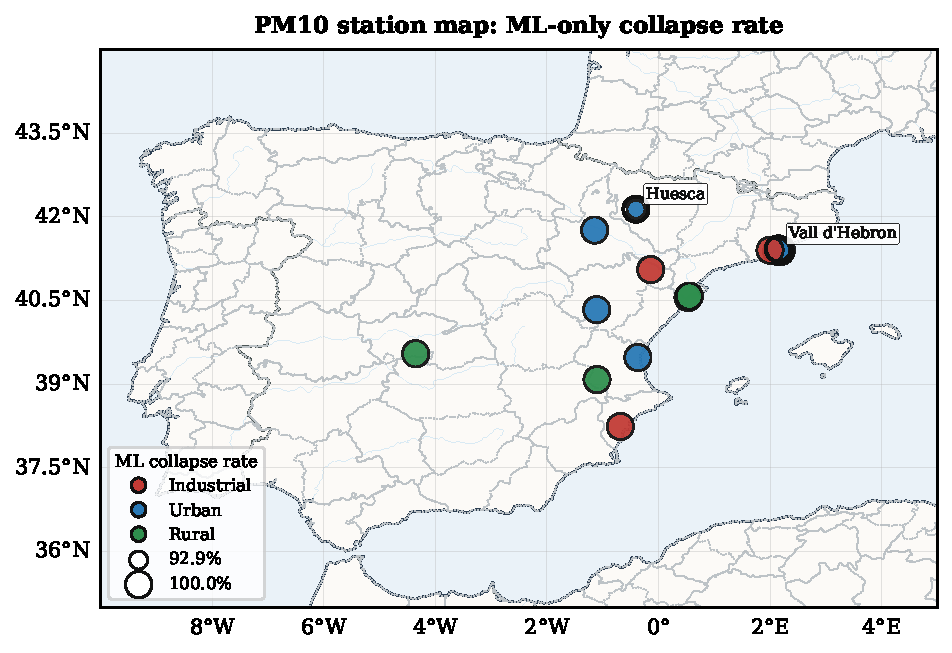
\includegraphics[width=\linewidth]{figures/station_map_ml_only_collapse_rate.pdf}
  \caption{Geographic distribution of the 17 MITECO stations. Marker colour denotes station type. Marker size denotes the ML-only collapse rate, computed over 14 model-horizon cells per station (2 direct ML models x 7 horizons). Fifteen stations show 14/14 collapsed ML cells; Huesca and Barcelona Vall d'Hebron show 13/14 due to one non-collapsed h=1 cell each.}
  \label{fig:station_map_ml_only}
\end{figure}

The results set an operational paradox: the direct ML forecasters can improve upon persistence in RMSE while producing trajectories that are substantially smoother than the observations. Interpreting performance therefore requires separating baseline-relative error reduction from the extent to which forecasts preserve day-to-day variability across horizons. The following discussion connects this decoupling to the squared-error objective and clarifies what it implies for episode-sensitive use.

